%!TEX program = xelatex
\documentclass[aspectratio=169]{beamer}
\usepackage[T1]{fontenc}
\usepackage{hyphenat}
\usepackage{geometry}
\usepackage{overpic}
\usepackage{tikz}

\usetikzlibrary{arrows, positioning}

%----------------------------------------
% Theme
%----------------------------------------

\graphicspath{{images/}}

\usetheme{utbm}
%\usetheme[illustration=cover]{utbm} % use cover.png/jpg/... for the title page

%\useinnertheme[illustration=cover]{utbm}
%\useoutertheme{utbm}
%\usecolortheme{utbm}

%----------------------------------------
% Informations
%----------------------------------------

\newcommand\TODO[1]{\textcolor{red}{TODO\@: #1}}

\title[Développement d’une plateforme de recueil de consentements RGPD]{Soutenance de stage}
\subtitle{Développement d’une plateforme de recueil de consentements RGPD}
\author{Nicolas Ballet}
\institute[UTBM]{Université de Technologie de Belfort Montbéliard}

\def\twodigits#1{\ifnum#1<10 0\fi\the#1}
\date[\the\year-\twodigits\month-\twodigits\day]{\today}

% PDF metadata informations
\keywords{Versusmind \hyp{} RGPD \hyp{} Consentement \hyp{} Signature numérique \hyp{} Cloud Microsoft Azure \newline Méthodologie Scrum \hyp{} Azure DevOps \hyp{} Angular \hyp{} Spring Boot \hyp{} Azure Functions}
\subject{J'ai pu, durant mon stage de fin d'études à Versusmind (Strasbourg), participer au développement d'un plateforme de recueil de consentement hébergée dans le cloud Microsoft Azure.\newline L'équipe dont j'ai fait partie, utilise la methode agile Scrum. J'ai aidé à terminer une refonte graphique, mais aussi, à faire face à des problèmatiques de montée en charge et d'optimisation. Le tout sur une base de tests d'intégrations à l'aide d'Azure DevOps.}

%----------------------------------------
% Document
%----------------------------------------
\begin{document}
\begin{frame}[plain,noframenumbering]
    \titlepage{}
\end{frame}
\begin{frame}{Sommaire}
    \tableofcontents
\end{frame}

\section{Contexte}
\begin{frame}
    \frametitle{Contexte}
    \framesubtitle{Entreprise}
    \begin{columns}
        \hfill
        \begin{column}{0.45\textwidth}
            \begin{center}
                \hfill
\includegraphics[width=1.0\textwidth]{versusmind.png}
            \end{center}
            \hfill \color{gray} Cabinet d'architecture numérique   
        \end{column}
        \begin{column}{0.5\textwidth}
            \begin{center}
                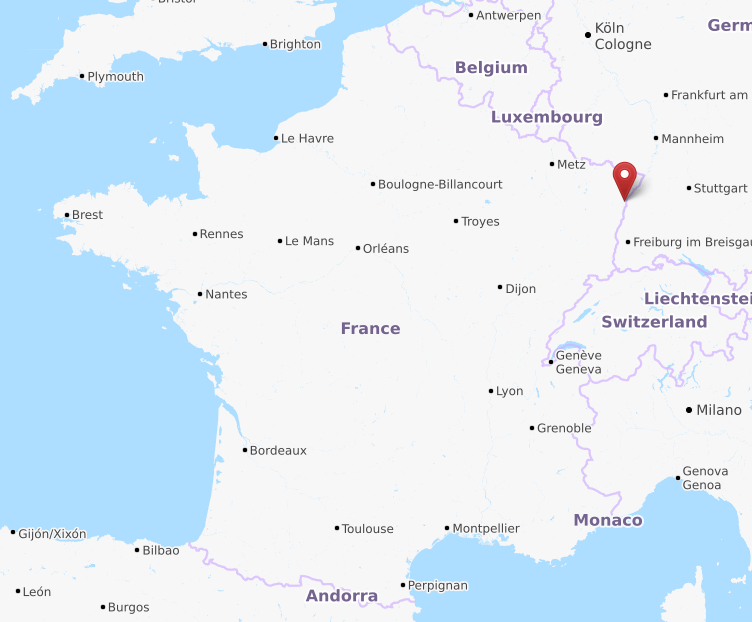
\includegraphics[width=1.0\textwidth]{strasbourg.png}
            \end{center}
        \end{column}
    \end{columns}
\end{frame}
\begin{frame}
    \frametitle{Contexte}
    \framesubtitle{RGPD}
    \begin{center}
        Règlement Général sur la Protection des Données
    \end{center}
    \begin{columns}
        \hfill
        \begin{column}{0.45\textwidth}
            \begin{enumerate}
                \item<1-> Uniformiser la réglementation au niveau européen
                \item<2-> Responsabiliser les entreprises
                \item<3-> Renforcer les droits des personnes
            \end{enumerate}
        \end{column}
        \begin{column}{0.5\textwidth}
            \begin{center}
                \onslide<1->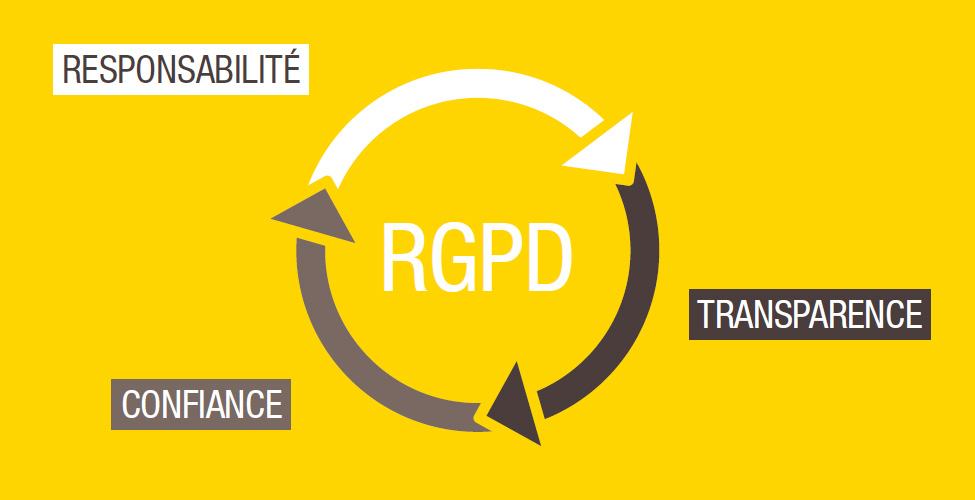
\includegraphics[width=1.0\textwidth]{RGPD.jpg}
            \end{center}
        \end{column}
    \end{columns}
\end{frame}
\begin{frame}
    \frametitle{Contexte}
    \framesubtitle{Central Consent Manager (CCM)}
    \begin{center}
        
\includegraphics[width=0.4\textwidth]{ccm_.png}
    \end{center}
    \begin{columns}
        \hfill
        \begin{column}{0.45\textwidth}
            \begin{enumerate}
                \item<1-> Requête sur le service de mentions pour un traitement
                \item<2-> Envoi des mentions d'informations
                \item<3-> Demande de consentement
                \item<4-> Confirmation
                \item<5-> Enregistrement du consentement
            \end{enumerate}
        \end{column}
        \begin{column}{0.5\textwidth}
            \begin{center}
                \onslide<1->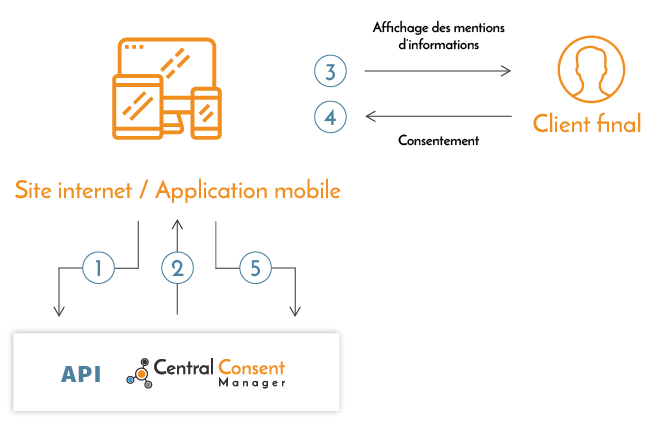
\includegraphics[width=1.0\textwidth]{ccm.png}
            \end{center}
        \end{column}
    \end{columns}
\end{frame}

\section{Refonte graphique}
\begin{frame}
    \frametitle{Refonte graphique}
    \framesubtitle{}
    \begin{columns}
        \hfill
        \begin{column}{0.45\textwidth}
            \begin{center}
                
\includegraphics[width=1.0\textwidth]{CSS_HTML.png}
            \end{center}
        \end{column}
        \begin{column}{0.5\textwidth}
            \begin{center}
                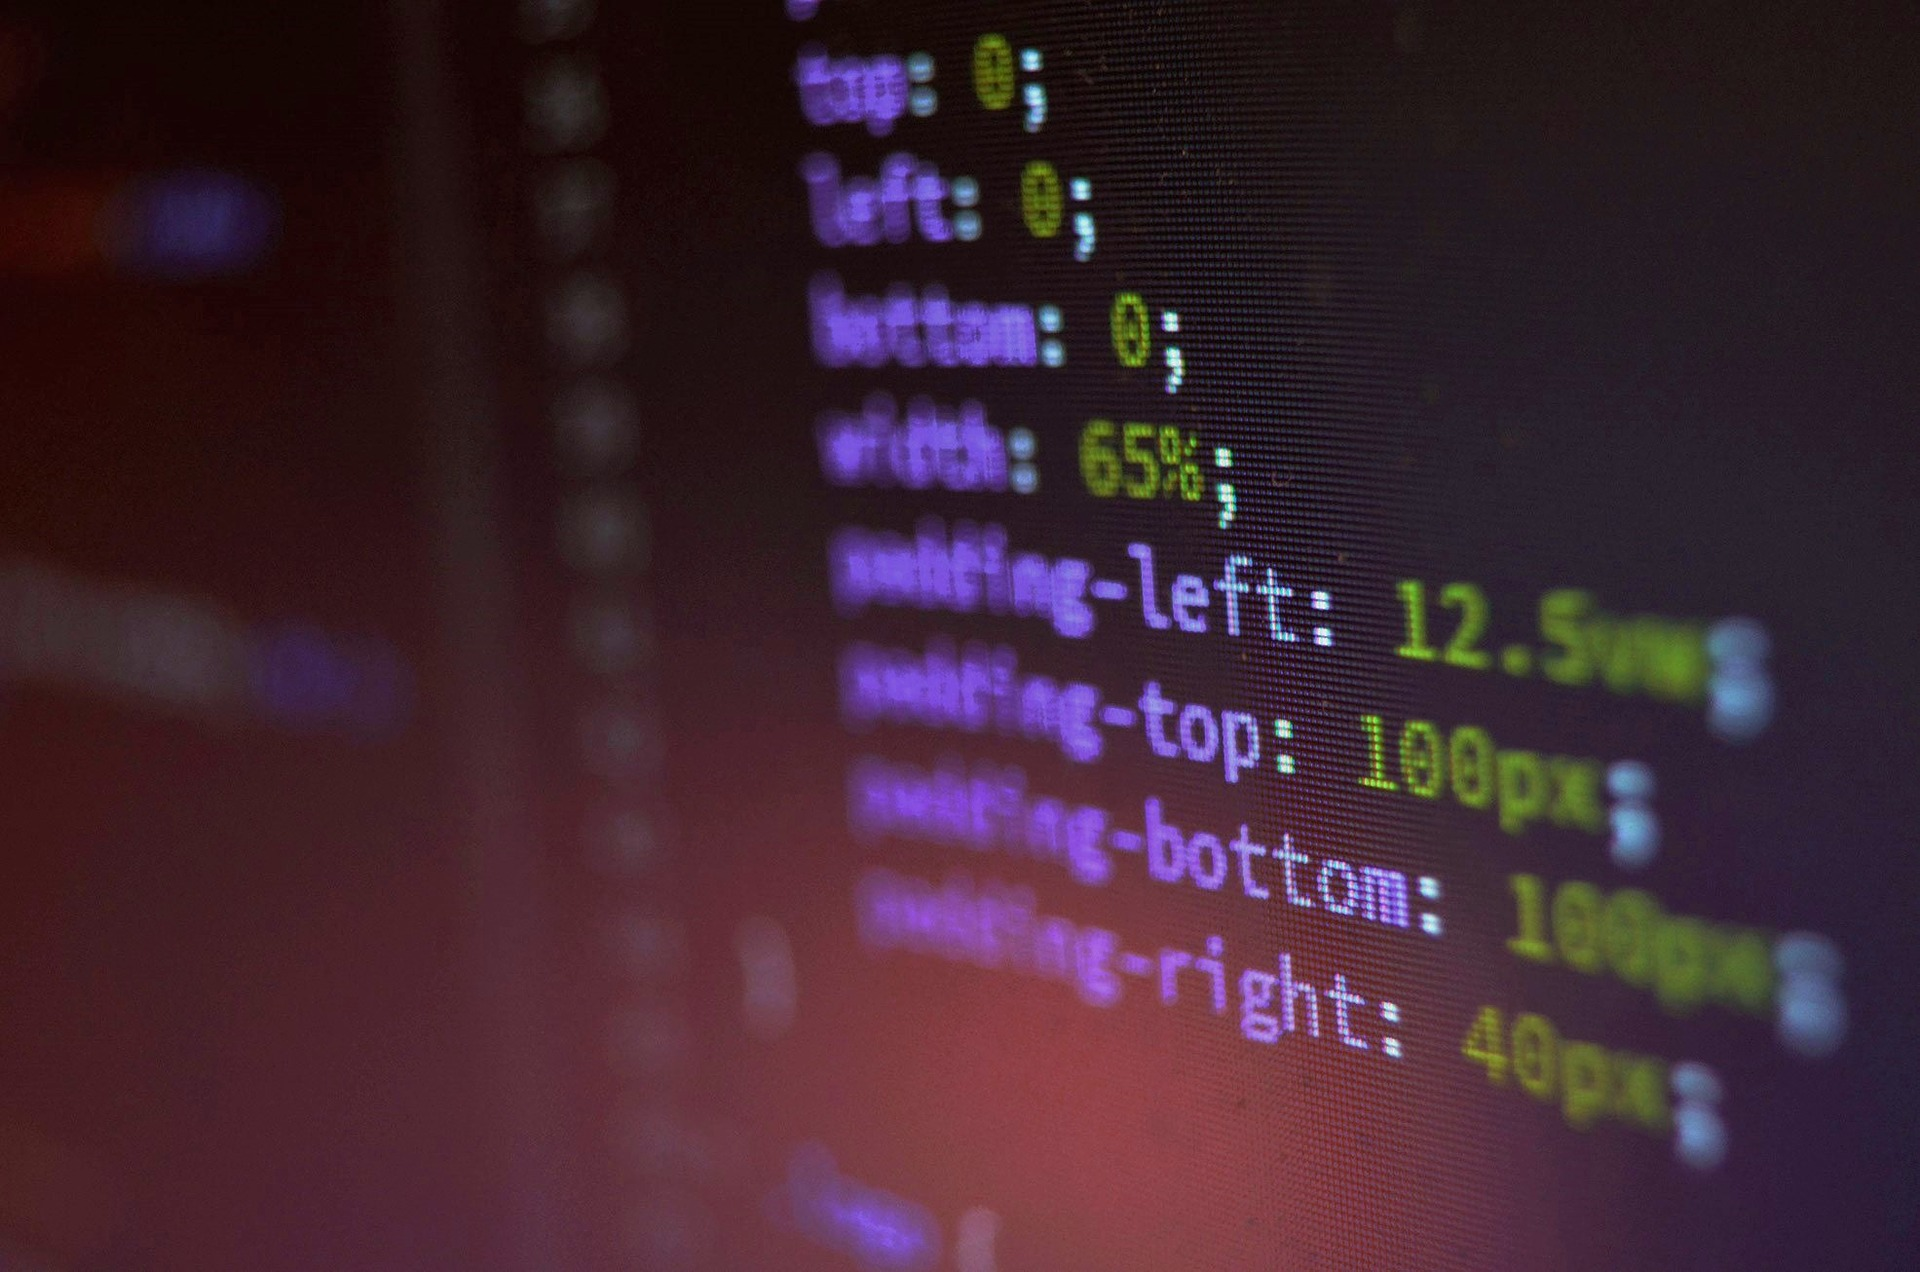
\includegraphics[width=1.0\textwidth]{code.jpg}
            \end{center}
        \end{column}
    \end{columns}
\end{frame}

\section{Optimisation}
\begin{frame}
    \frametitle{Optimisation}
    \framesubtitle{}
    \begin{center}
        \begin{tikzpicture}
            % nodes
            \node (api) at (1, 1.8) {
\includegraphics[width=0.1\textwidth]{website.png}};
            \node [above=0 of api] {API};
            \node (front) at (1, -1.8) {\begin{overpic}[width=0.1\textwidth]{website.png}
                    \put(60, -30){
\includegraphics[scale=.08]{ccm_logo.png}}
                \end{overpic}};
            \node [above=0 of front] {Front-end};
            \node (back) at (6, 0) {
\includegraphics[width=0.1\textwidth]{server.png}};
            \node [above=0 of back] {Back-end};
            \onslide<2>\node (function) at (12, 1.8) {
\includegraphics[width=0.1\textwidth]{cloud.png}};
            \onslide<2>\node [above=0 of function] {Azure Function};
            \onslide<1-2>\node (ejbca) at (12, -2) {
\includegraphics[width=0.2\textwidth]{ejbca.png}};

            % arrows
            \onslide<1-2>\draw[ultra thick, ->,>=stealth] (api) -- (back);
            \onslide<1-2>\draw[ultra thick, ->,>=stealth] (front) -- (back);
            \onslide<1>\draw[ultra thick, ->,>=stealth] (back) -- (ejbca);
            \onslide<2>\draw[ultra thick, double, <->,>=stealth] (back) -- node[above, sloped] {Service Bus} (function);
            \onslide<2>\draw[ultra thick, ->,>=stealth] (function) -- (ejbca);

        \end{tikzpicture}
    \end{center}
\end{frame}

\section{Conclusion}
\begin{frame}
    \frametitle{Conclusion}
    \framesubtitle{}
    \begin{itemize}
        \item 
        \item Cool
        \item Good CDI
    \end{itemize}
\end{frame}
\begin{frame}[plain,noframenumbering]
    \utbmclosingframe{Avez vous des questions ?}
\end{frame}
\end{document}
